% Section 5 - Integrating Simulink models
% Roberto Masocco <roberto.masocco@uniroma2.it>
% Alessandro Tenaglia <alessandro.tenaglia@uniroma2.it>
% June 5, 2024

% ### Integrating Simulink models ###
\section{Integrating Simulink models}
\graphicspath{{figs/section5/}}

% --- Model creation ---
\begin{frame}{Model creation}
	Create the model paying attention to data types.\\
  \bigskip
	Define inputs as \textbg{Inport blocks} and name them.\\
  \bigskip
	Define outputs as \textbg{Outport blocks} and name them.\\
  \bigskip
  Compiled \textbg{shared libraries} can then be loaded by a \textbg{SimulinkWrapperGAM}.
	\vspace{0.5cm}
	\begin{figure}
		\centering
		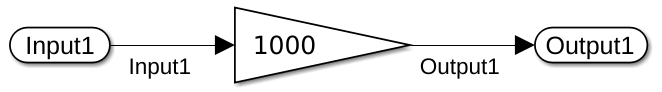
\includegraphics[scale=0.4]{Model.png}
		\caption{Basic Simulink model example.}
		\label{fig:model}
	\end{figure}
\end{frame}

% --- Parameters ---
\begin{frame}{Parameters}
	Paramters can be:
	\begin{itemize}
		\item \textbg{static}, no longer modifiable after the code generation;
		\item \textbg{tunable}, so they can be modified at runtime.
	\end{itemize}
	\vspace{0.5cm}
	\begin{figure}
		\centering
		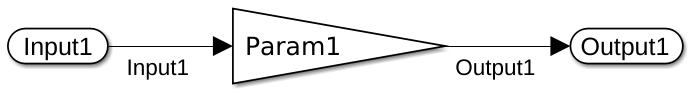
\includegraphics[scale=0.4]{ModelParam.png}
		\caption{Basic Simulink model with a tunable parameter.}
		\label{fig:model_param}
	\end{figure}
\end{frame}

% --- Code generation ---
\begin{frame}{Code generation}
	\begin{figure}
		\centering
		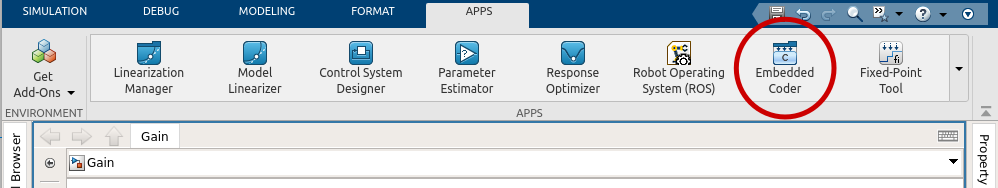
\includegraphics[width=\textwidth]{Embedded.png}
		\label{fig:embedded}
		\caption{Embedded Coder app location.}
	\end{figure}
\end{frame}
\begin{frame}{Code generation}
	\begin{figure}
		\centering
		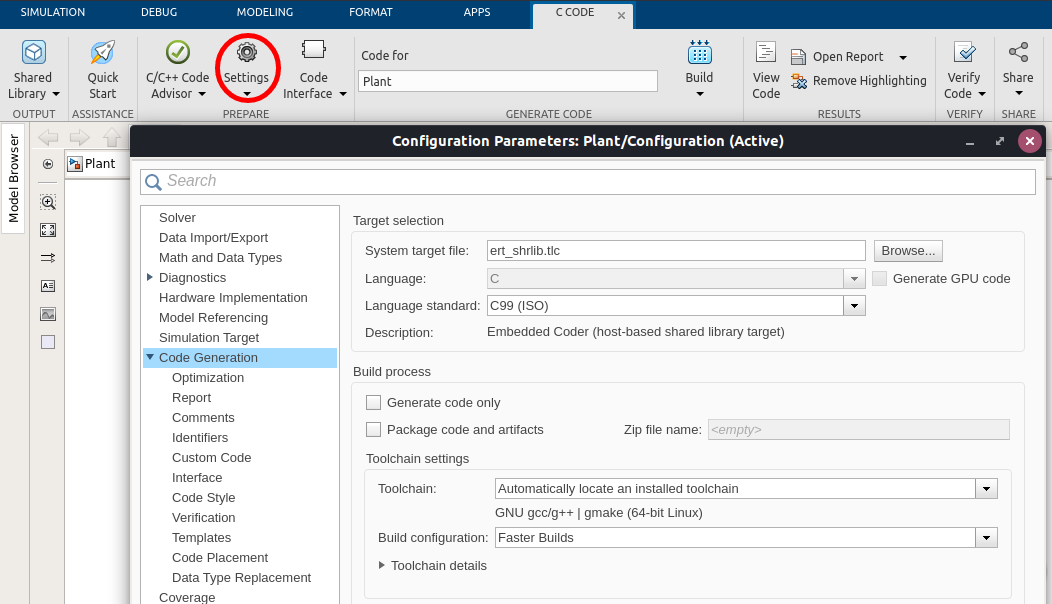
\includegraphics[scale=.27]{Settings.png}
		\caption{Code generation settings.}
		\label{fig:settingd}
	\end{figure}
\end{frame}
\begin{frame}{Code generation}
	\begin{figure}
		\centering
		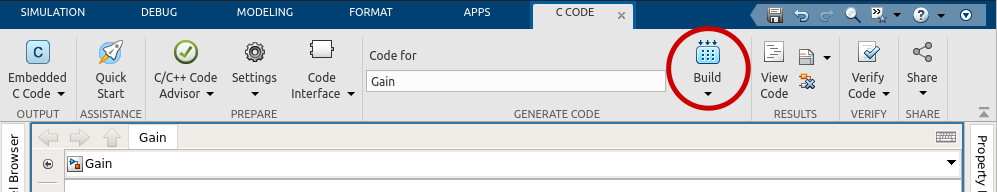
\includegraphics[width=\textwidth]{Build.png}
		\caption{Build button location.}
		\label{fig:build}
	\end{figure}
\end{frame}

% --- Configuration file: SimulinkWrapperGAM ---
\begin{frame}[fragile]{Configuration file: SimulinkWrapperGAM}
	\begin{columns}\column{.8\textwidth}
		\begin{lstlisting}[style=small, language = cfg, caption=SimulinkWrapperGAM configuration structure (brackets due to space constraints).]
+GAMGain = {
    Class = SimulinkWrapperGAM
    Library = Gain.so // Library name
    SymbolPrefix = Gain // Model name
    InputSignals = {
        Input1 = {
            DataSource = DDB1
            Type = int32}}
    OutputSignals = {
        Output1 = {
            DataSource = DDB1
            Type = int32}}
    Parameters = {
        Param1 = (int32) 1000}
}\end{lstlisting}
	\end{columns}
\end{frame}

% --- Example: Control system ---
\begin{frame}{Example: Control system}
	\begin{figure}
		\centering
		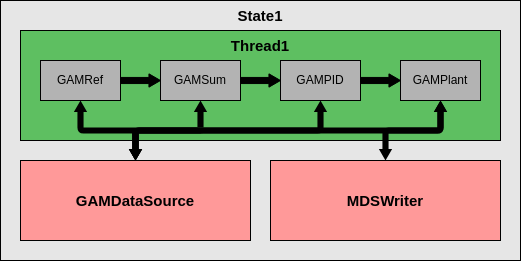
\includegraphics[scale=.67]{ControlSystem.png}
		\caption{Control system MARTe app operational scheme.}
		\label{fig:control}
	\end{figure}
\end{frame}
